\documentclass[aspectratio=169,11pt]{beamer}

% Match the visual language of the SIAM Waves talk.
\usetheme{Boadilla}
\usecolortheme{seahorse}
\useinnertheme{rectangles}
\useoutertheme{infolines}

\setbeamercolor{structure}{fg=blue!55!black}
\setbeamercolor{title}{fg=white,bg=blue!55!black}
\setbeamercolor{frametitle}{fg=blue!55!black}
\setbeamercolor{block title}{bg=blue!12,fg=blue!55!black}
\setbeamercolor{block body}{bg=blue!4}
\setbeamertemplate{navigation symbols}{}
\setbeamerfont{frametitle}{series=\bfseries,size=\large}
\setbeamerfont{title}{series=\bfseries,size=\Large}

\usepackage[T1]{fontenc}
\usepackage[utf8]{inputenc}
\DeclareFontShape{T1}{cmss}{b}{n}{<->ssub*cmss/bx/n}{}
\usepackage{amsmath, amssymb, bm}
\usepackage{graphicx}
\usepackage{xcolor}
\usepackage{tikz}
\usetikzlibrary{arrows.meta,calc,decorations.pathmorphing,patterns}
\usepackage{pgfplots}
\pgfplotsset{compat=1.18}
\usepackage{hyperref}
\hypersetup{colorlinks=true,urlcolor=blue!55!black}

% ---------- Macros ----------
\newcommand{\R}{\mathbb{R}}
\newcommand{\uu}{\bm{u}}
\newcommand{\pp}{p}
\newcommand{\Rey}{\mathrm{Re}}
\newcommand{\nuu}{\nu}
\newcommand{\tmark}[1]{\hfill{\scriptsize\textcolor{gray}{#1}}}

% Uncomment if you want speaker notes:
% \usepackage{pgfpages}
% \setbeameroption{show notes on second screen=right}

\title[Turbulence: what is it?]{What is turbulence?}
\subtitle{Key features, examples, and why it matters}
\author[Miller]{Laura A. Miller}
\institute[UArizona]{Department of Mathematics, University of Arizona}
\date{}

\begin{document}

% ---------------- Title ----------------
\begin{frame}[plain]
  \begin{beamercolorbox}[sep=10pt,center]{title}
    {\bfseries\Large What is turbulence?}\\[3pt]
    {\normalsize Key features, examples, and why it matters}
  \end{beamercolorbox}
  \vspace{1.35em}
  \begin{columns}[T,onlytextwidth]
  \begin{column}{0.55\textwidth}
    \textbf{\large Laura A. Miller}\\[4pt]
    Department of Mathematics\\
    University of Arizona\\[12pt]
    {\small IBFE Tutorials}
  \end{column}
  \begin{column}{0.45\textwidth}
    \begin{block}{A working viewpoint}
    Turbulence is recognized through a collection of dynamical signatures, not one universal checklist.
    \end{block}
  \end{column}
  \end{columns}
  \vfill
  {\scriptsize Adapted from a \href{https://doi.org/10.52843/cassyni.hrpvdf}{lecture by Steven L. Brunton}.}
  \\[2pt]{\tiny AI tools were used to assist with formatting, organization, and clarification of the instructor's original notes.}
  \note{
  Goal: build intuition + a math-friendly entry point.
  No single definition; use a set of hallmark features + canonical examples.
  }
\end{frame}

% ---------------- Motivation ----------------
\begin{frame}{Why turbulence fascinates us}
\vspace{-0.3em}
\begin{itemize}
  \item Turbulence shows up in \textbf{art} and \textbf{language}: roiling, churning, turbulent.
  \item We have strong intuition for ``turbulent'' vs ``not,'' but a single universal definition is hard.
  \item So: we focus on \textbf{key features} and \textbf{canonical examples}.
\end{itemize}

\centering
\includegraphics[width=0.45\textwidth]{pictures/5-1/da-Vinci.png}
\vfill
  \hfill {\scriptsize Leonardo da Vinci, \emph{Studies of water}, c.~1510--1512 (Royal Collection, public domain).}
\end{frame}

\begin{frame}{Turbulence in art: Van Gogh}

\centering
\includegraphics[width=0.55\textwidth]{pictures/5-1/Van_Gogh_Starry_Night.jpg}
\vfill
  \hfill {\scriptsize Vincent van Gogh, \emph{The Starry Night} (1889), MoMA (public domain).}
\end{frame}

% ---------------- Fingerprint ----------------
\begin{frame}{A practical ``fingerprint'' of turbulence}
\textbf{A useful operational fingerprint is that turbulent flows are typically:}
\begin{enumerate}
  \item \textbf{Three-dimensional} (3D vortical motion),
  \item \textbf{Multi-scale} in space and time (big eddies $\rightarrow$ small eddies),
  \item \textbf{Unsteady} (time-evolving),
  \item \textbf{Mixing} and strongly transporting scalar/particles.
\end{enumerate}

\vspace{0.7em}
\textbf{Mental experiment:} add dye upstream $\Rightarrow$ rapid stretching and folding $\Rightarrow$ enhanced mixing.  This is a diagnostic, not a formal definition.

\end{frame}

% ---------------- 2D caveat ----------------
\begin{frame}{A note on 2D vs 3D turbulence}
\begin{itemize}
  \item In 3D turbulence, kinetic energy is typically transferred toward smaller scales and ultimately dissipated by viscosity.
  \item Idealized 2D turbulence has two inviscid quadratic invariants: energy tends upscale, while enstrophy tends downscale.
  \item Rotating or stratified geophysical flows can be \textbf{quasi-2D}; finite thickness, friction, and wave dynamics modify the ideal picture.
\end{itemize}

\vspace{0.25em}
\centering
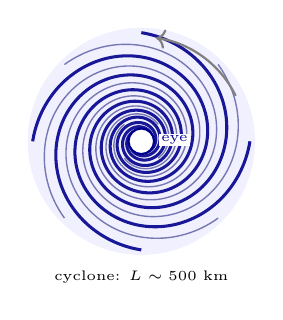
\begin{tikzpicture}[x=0.74cm,y=0.74cm]
  \fill[blue!6] (0,0) circle (1.95);
  % logarithmic spiral rain bands
  \foreach \s in {0,90,180,270}{%
    \draw[blue!55!black,line width=1.1pt,opacity=0.9,samples=300,smooth,variable=\t,domain=0:900]
      plot ({0.149*exp(0.0028*\t)*cos(\t+\s)},{0.149*exp(0.0028*\t)*sin(\t+\s)});
  }
  \foreach \s in {45,135,225,315}{%
    \draw[blue!40!black,line width=0.5pt,opacity=0.5,samples=220,smooth,variable=\t,domain=360:900]
      plot ({0.149*exp(0.0028*\t)*cos(\t+\s)},{0.149*exp(0.0028*\t)*sin(\t+\s)});
  }
  % eye
  \fill[white] (0,0) circle (0.22);
  \draw[blue!55!black,thick] (0,0) circle (0.22);
  \node[font=\tiny,blue!55!black,anchor=west,fill=white,inner sep=0.7pt] at (0.30,0.02) {eye};
  % sense of rotation
  \draw[->,gray,thick] (1.62,0.78) arc (26:82:1.80);
  \node[font=\tiny,anchor=north] at (0,-2.05) {cyclone: $L\sim 500$ km};
\end{tikzpicture}

{\scriptsize Schematic (instructor's course notes).}

\end{frame}

% ---------------- Course notes pointer ----------------
\begin{frame}{A recommended reference (from the lecture)}
\begin{itemize}
  \item \href{http://profs.sci.univr.it/~zuccher/downloads/FD-MAE553-Smits.pdf}{Lex Smits (Princeton): \textbf{MAE 553 Viscous Flows and Turbulence} notes.}
  \item Use as a companion source for canonical flows and experimental intuition.
\end{itemize}

\vspace{0.8em}
\centering
\includegraphics[width=0.5\textwidth]{pictures/5-1/lectures-smit.png}

{\scriptsize Title page of A. J. (Lex) Smits, \emph{MAE 553: Viscous Flows and Turbulence} lecture notes (Princeton University).}

\end{frame}

% ---------------- Boundary layer simulation ----------------
\begin{frame}{Example: a turbulent boundary layer (simulation)}
\begin{itemize}
  \item High-fidelity simulation of a developing boundary layer (think: flow over a wing/car).
  \item Observe: \textbf{3D}, \textbf{unsteady}, \textbf{multi-scale}, \textbf{mixing}.
\end{itemize}

\vspace{0.8em}

\centering
\href{https://www.youtube.com/watch?v=4KeaAhVoPIw}{\color{blue}\underline{3D Simulation (YouTube)}}
\end{frame}



% ---------------- Multiscale structure ----------------
\begin{frame}{Hallmark: multi-scale structure}
\begin{itemize}
  \item ``Zoom in anywhere'' $\Rightarrow$ you see more structure.
  \item Multi-scale content is a quick visual diagnostic of turbulence.
\end{itemize}

\vspace{0.7em}
\textbf{Fun aside (from lecture):} blockbuster explosions look ``high budget'' when they show many scales.

\centering
\includegraphics[width=0.5\textwidth]{pictures/5-1/explosion.png}

\hfill
{\scriptsize Still from \emph{Oppenheimer} (dir. C. Nolan, Universal Pictures, 2023); shown for educational commentary, rights reserved by the studio.}

\end{frame}

% ---------------- Ocean/atmosphere ----------------
\begin{frame}{Turbulence at planetary scales}
\begin{itemize}
  \item Ocean currents and atmospheric patterns are highly turbulent.
  \item Turbulent transport $\Rightarrow$ global mixing of heat, salt, nutrients, pollutants.
\end{itemize}

\vspace{0.6em}
\centering
\includegraphics[width=0.5\textwidth]{pictures/5-1/ocean-mix.jpg}
  \hfill

{\scriptsize Photo: Kent Smith, Gulf of Alaska (2007), glacial meltwater meeting ocean water.}
\end{frame}

% ---------------- Rayleigh-Bénard + chaos ----------------
\begin{frame}{Rayleigh--B\'enard convection and chaos}
\begin{itemize}
  \item Heated from below, cooled from above $\Rightarrow$ convective instability.
  \item Unsteady + multi-scale + mixing (often used to motivate chaotic dynamics).
  \item Historical link: Lorenz (1963) studied simplified models of convective rolls.
\end{itemize}

\vspace{0.5em}

\centering
\href{https://www.youtube.com/watch?v=YkN6F6LJzGU}{\color{blue}\underline{3D Simulation (YouTube)}}

\end{frame}

% ---------------- Navier–Stokes entry ----------------
\begin{frame}{Mathematical entry point: incompressible Navier--Stokes}
\begin{align*}
\frac{\partial\uu}{\partial t} + (\uu\cdot\nabla)\uu &= -\nabla \pp + \frac{1}{\Rey}\, \Delta \uu,\\
\nabla\cdot\uu &= 0.
\end{align*}

\[
\mathbf{u}(\mathbf{x},t)=
\begin{bmatrix}
u(\mathbf{x},t)\\
v(\mathbf{x},t)\\
w(\mathbf{x},t)
\end{bmatrix}
\]


\begin{itemize}
  \item $\uu(\bm{x},t)\in\R^3$ is a 3-component velocity field.
  \item Rich behavior emerges as parameters/forcing/geometry change.
\end{itemize}

\end{frame}

% ---------------- Reynolds number ----------------
\begin{frame}{Reynolds number: a control knob for complexity}
\begin{columns}[T,onlytextwidth]
  \begin{column}{0.58\textwidth}
    \begin{itemize}
      \item For chosen characteristic scales $U$ and $L$, the \textbf{Reynolds number} compares inertial and viscous effects:
      \[
        \Rey \sim \frac{U L}{\nuu}.
      \]
      \item It is a \textbf{control parameter}, but geometry, forcing, roughness, and disturbances also determine the observed state.
      \item In high-$\Rey$, 3D, locally isotropic turbulence, Kolmogorov scaling estimates $L/\eta\sim \Rey_L^{3/4}$; this is not a universal one-to-one law.
    \end{itemize}
  \end{column}

  \begin{column}{0.42\textwidth}
    \centering
    \includegraphics[width=0.62\linewidth]{pictures/5-1/flow-cylinder.png}

    {\scriptsize Flow regimes past a cylinder; after S. Vogel, \emph{Life in Moving Fluids}, 2nd ed. (Princeton Univ.\ Press, 1994) (figure number to confirm).}
  \end{column}
\end{columns}
\end{frame}


% ---------------- Drag vs Re ----------------
\begin{frame}{Drag depends strongly on Reynolds number}
\begin{itemize}
  \item As flow regime changes with $\Rey$, the drag coefficient can change dramatically.
  \item Implication: ``just changing speed'' can change force laws in big ways.
\end{itemize}

\vspace{0.3em}
    \centering
    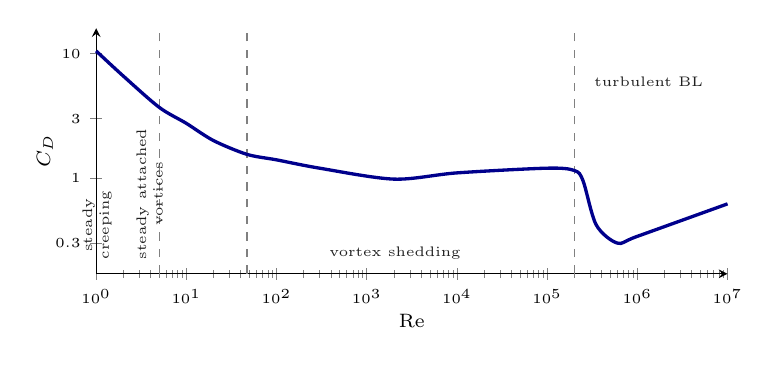
\begin{tikzpicture}
    \begin{axis}[
      width=9.6cm, height=4.7cm,
      xmode=log, ymode=log,
      xmin=1, xmax=1e7, ymin=0.17, ymax=16,
      xlabel={$\Rey$}, ylabel={$C_D$},
      xlabel style={font=\scriptsize,yshift=3pt},
      ylabel style={font=\scriptsize,yshift=-6pt},
      ytick={0.3,1,3,10}, yticklabels={$0.3$,$1$,$3$,$10$},
      xtick={1,1e1,1e2,1e3,1e4,1e5,1e6,1e7},
      tick label style={font=\tiny},
      axis lines=left,
      clip=false,
      ]
      % regime boundaries
      \draw[gray,dashed] (axis cs:5,0.17) -- (axis cs:5,16);
      \draw[gray,dashed] (axis cs:47,0.17) -- (axis cs:47,16);
      \draw[gray,dashed] (axis cs:2e5,0.17) -- (axis cs:2e5,16);
      % qualitative C_D(Re) for a circular cylinder
      \addplot[blue!55!black,very thick,smooth] coordinates {
        (1,10.5) (2,6.6) (5,3.7) (10,2.75) (20,2.0) (47,1.55)
        (1e2,1.4) (3e2,1.2) (2e3,0.98) (1e4,1.1) (1e5,1.20)
        (2e5,1.15) (2.5e5,0.95) (3.5e5,0.42) (6e5,0.30)
        (1e6,0.34) (1e7,0.62)
      };
      % regime labels
      \node[rotate=90,anchor=south west,align=center,font=\tiny,gray!25!black]
        at (axis cs:1.9,0.185) {steady\\creeping};
      \node[rotate=90,anchor=south west,align=center,font=\tiny,gray!25!black]
        at (axis cs:7,0.185) {steady attached\\vortices};
      \node[anchor=south west,font=\tiny,gray!25!black] at (axis cs:3e2,0.185) {vortex shedding};
      \node[anchor=south west,font=\tiny,gray!25!black] at (axis cs:2.6e5,4.5) {turbulent BL};
    \end{axis}
    \end{tikzpicture}

{\scriptsize Drag coefficient of a circular cylinder versus Reynolds number with flow regimes. Schematic (instructor's course notes).}

\end{frame}

% ---------------- Galileo aside ----------------
\begin{frame}{Aside: Galileo's ball drop through multiple regimes}
\begin{columns}[T,onlytextwidth]
  \begin{column}{0.55\textwidth}
\begin{itemize}
  \item Falling ball accelerates $\Rightarrow$ effective $\Rey$ increases during the fall.
  \item Drag force can be highly unsteady and regime-dependent.
  \item Heavy objects: turbulent drag may be negligible relative to weight; light objects: not.
  \item The gravitational field $g$ may be nearly constant, while the ball's acceleration need not remain $g$ once drag is appreciable.
\end{itemize}
\end{column}
\begin{column}{0.45\textwidth}
    \centering
    \includegraphics[width=0.75\linewidth]{pictures/5-1/galileo.jpg}
     \vfill
    \raggedleft{\scriptsize Portrait of Galileo Galilei (public domain); the legendary experiment at Pisa.}
  \end{column}
\end{columns}
\end{frame}

% ---------------- Osborne Reynolds ----------------
\begin{frame}{Why ``Reynolds''? Pipe-flow experiments (1883)}
\small
\begin{itemize}
  \item Osborne Reynolds observed changes in pipe flow as speed and disturbance conditions varied:
  \begin{itemize}
    \item laminar (layered, steady),
    \item transitional,
    \item turbulent (roiling, disordered).
  \end{itemize}
  \item The laminar solution exists at every $\Rey$; pipe transition is subcritical and depends on finite-amplitude disturbances.
  \item Pipe flow remains a core engineering problem: pumping water, sewage, and process fluids efficiently.
  \item Textbooks quote $\Rey_D\approx 2300$ for the onset of transition in pipes; Reynolds (1883) found transition near $\Rey\approx 13{,}000$ with a disturbed inlet and could keep flow laminar to far higher $\Rey$ with care. Deck 5-4 discusses the modern value $\Rey_D\approx 2040$.
\end{itemize}

\vspace{0.1em}
\centering
    \includegraphics[width=0.26\linewidth]{pictures/5-1/04-reynolds.jpg}
  \hfill

{\scriptsize Apparatus and dye-filament plate from O. Reynolds, \emph{Phil.\ Trans.\ R. Soc.\ Lond.} \textbf{174} (1883), 935--982 (public domain).}
\end{frame}

\begin{frame}{Transition to turbulence}
\begin{itemize}
  \item A classical experiment is to inject dye into a tube to visualize the flow.
  \item As $\Rey$ and/or disturbance amplitude increase, the dye filament may become unsteady and then turbulent.
  \item A single critical value is not universal: inlet noise, roughness, and protocol matter.
\end{itemize}

\vspace{0.8em}

\centering
\href{https://youtu.be/BBiR6FWmyv4}{\color{blue}\underline{Pipe flow transition to turbulence (YouTube)}}
\end{frame}
% ---------------- Turbulence is not random ----------------
\begin{frame}{Turbulence is not ``random'': coherent structures}
\begin{itemize}
  \item Turbulence has stochastic aspects, but it is not structureless noise.
  \item \textbf{Coherent structures} (organized patterns) can persist within complex flows.
  \item Similar large-scale patterns can appear across wildly different Reynolds numbers.
\end{itemize}

\vspace{0.5em}
\centering
    \includegraphics[width=0.9\linewidth]{pictures/5-1/vonkarman.png}
      \hfill

{\scriptsize M. Van Dyke, \emph{An Album of Fluid Motion} (Parabolic Press, 1982).}

\end{frame}

% ---------------- Brown & Roshko mixing layers ----------------
\begin{frame}{Mixing layers: laminar vs turbulent share patterns}
\begin{columns}[T,onlytextwidth]
  \begin{column}{0.5\textwidth}
    \begin{itemize}
      \item Classic mixing-layer images show:
      \begin{itemize}
        \item Bottom: low-$\Rey$ (laminar), \item Middle: intermediate-$\Rey$ (transitional), and \item Top: high-$\Rey$ (turbulent).
        \end{itemize}
        \item All cases share recognizable, coherent structures.
        \item Turbulence adds scales and distortion, but does not erase organization.
      \end{itemize}
  \end{column}

  \begin{column}{0.45\textwidth}
    \centering
    \includegraphics[width=0.72\linewidth]{pictures/5-1/mixing-layers.png}

    \vfill
    \raggedleft{\scriptsize Shadowgraphs of a plane mixing layer at increasing Reynolds number; G. L. Brown \& A. Roshko, \emph{J. Fluid Mech.} \textbf{64}, 775--816 (1974); reproduced in Van Dyke, \emph{An Album of Fluid Motion}.}
  \end{column}
\end{columns}
\end{frame}


% ---------------- Intermittency ----------------
\begin{frame}{Another hallmark: intermittency}
\begin{itemize}
  \item Turbulence can be \textbf{patchy} in space/time:
  \begin{itemize}
    \item turbulent region $\rightarrow$ calm region $\rightarrow$ turbulent again.
  \end{itemize}
  \item Picture: smoke plume, clouds in the boundary layer, bursts of turbulence.
  \item Useful concept: an ``intermittency function'' that switches on/off turbulence.
\end{itemize}

\vspace{0.5em}
\centering
    \includegraphics[width=0.55\linewidth]{pictures/5-1/intermitancy.png}

    \vfill
    {\footnotesize Source: Smith and Smits, 1988.}

\end{frame}

\begin{frame}{Intermittency in pipe flow}
\centering
    \includegraphics[width=0.4\linewidth]{pictures/5-1/local-turbulence.png}
    
\vfill
    {\footnotesize Source: Nikitin, N. \& Pimanov, V.. (2015). Numerical study of localized turbulent structures in a pipe. Fluid Dynamics. 50. 655-664.} 
    \end{frame}
% ---------------- Canonical flows ----------------
\begin{frame}{How we handle complexity: canonical flows}
\begin{columns}[T,onlytextwidth]
  \begin{column}{0.5\textwidth}
    \begin{itemize}
      \item Canonical flows: isotropic turbulence, wall-bounded flows, boundary layers, mixing layers, pipe flow, channel flow, cavity flow, wakes, jets.
      \item Strategy: distill turbulence into idealized building blocks.
      \item Real systems combine many of these (boundary layer + wake + jet + mixing layer).
    \end{itemize}
  \end{column}

  \begin{column}{0.48\textwidth}
    \centering
    \includegraphics[width=0.58\linewidth]{pictures/5-1/album.png}

    {\scriptsize M. Van Dyke, \emph{An Album of Fluid Motion} (Parabolic Press, 1982), cover.}
  \end{column}
\end{columns}
\end{frame}


% ---------------- Examples: wakes, mixing layers, jets ----------------
\begin{frame}{Examples of canonical flows and why they matter}
\begin{columns}[T,onlytextwidth]
\column{0.33\textwidth}
\textbf{Wakes}
\begin{itemize}
  \item drag and unsteady forces
  \item vehicles, trains, projectiles, fish, birds
\end{itemize}

 \vspace{0.5em}
\centering
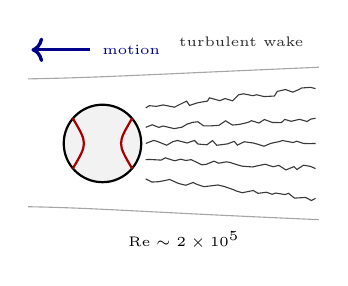
\begin{tikzpicture}[x=0.82cm,y=0.82cm]
  % outer streamlines
  \draw[gray!70] (0.1,2.60) .. controls (1.2,2.62) and (1.8,2.66) .. (4.6,2.78);
  \draw[gray!70] (0.1,0.62) .. controls (1.2,0.60) and (1.8,0.54) .. (4.6,0.42);
  % ball
  \draw[thick,fill=gray!10] (1.25,1.60) circle (0.60);
  \draw[red!65!black,thick] (0.79,1.21) .. controls (1.02,1.60) .. (0.79,1.99);
  \draw[red!65!black,thick] (1.71,1.21) .. controls (1.48,1.60) .. (1.71,1.99);
  % motion to the left
  \draw[->,very thick,blue!55!black] (1.05,3.05) -- (0.15,3.05);
  \node[font=\tiny,anchor=west,blue!55!black] at (1.10,3.05) {motion};
  % turbulent wake behind (to the right)
  \foreach \y/\g in {1.05/-0.30,1.35/-0.14,1.60/0.0,1.85/0.14,2.15/0.30}{%
    \draw[gray!45!black,decorate,decoration={random steps,segment length=2.4pt,amplitude=1.1pt}]
      (1.92,\y) -- (4.55,{\y+\g});
  }
  \node[font=\tiny,anchor=south,gray!35!black] at (3.4,2.95) {turbulent wake};
  \node[font=\tiny,anchor=west] at (1.5,0.10) {$\Rey\sim2\times10^{5}$};
\end{tikzpicture}

{\scriptsize Schematic (instructor's course notes).}

\column{0.33\textwidth}
\textbf{Mixing layers}
\begin{itemize}
  \item shear-driven mixing
  \item ocean waves, atmospheric inversion layers
\end{itemize}

 \vspace{0.5em}
\centering
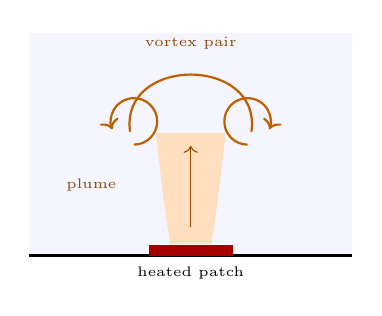
\begin{tikzpicture}[x=0.82cm,y=0.82cm]
  \fill[blue!4] (0,0) rectangle (5,3.45);
  % rising plume stem, widening upward
  \fill[orange!25]
    (2.18,0.18) .. controls (2.08,0.85) .. (1.96,1.90)
    -- (3.04,1.90) .. controls (2.92,0.85) .. (2.82,0.18) -- cycle;
  % mushroom cap
  \draw[orange!75!black,thick]
    (1.56,1.92) .. controls (1.40,3.10) and (3.60,3.10) .. (3.44,1.92);
  % counter-rotating vortex pair
  \draw[->,orange!75!black,thick] (1.62,1.72) arc (-90:200:0.36);
  \draw[->,orange!75!black,thick] (3.38,1.72) arc (270:-20:0.36);
  \draw[->,orange!60!black] (2.5,0.45) -- (2.5,1.70);
  % heated patch and floor
  \draw[very thick] (0,0) -- (5,0);
  \fill[red!65!black] (1.85,0) rectangle (3.15,0.17);
  \node[font=\tiny,anchor=north] at (2.5,-0.02) {heated patch};
  \node[font=\tiny,anchor=south,orange!55!black] at (2.5,3.05) {vortex pair};
  \node[font=\tiny,anchor=east,orange!55!black] at (1.50,1.10) {plume};
\end{tikzpicture}

{\scriptsize Schematic (instructor's course notes).}

\column{0.33\textwidth}
\textbf{Jets}
\begin{itemize}
  \item thrust and power
  \item noise and quality-of-life impacts
\end{itemize}

 \vspace{0.5em}
\centering
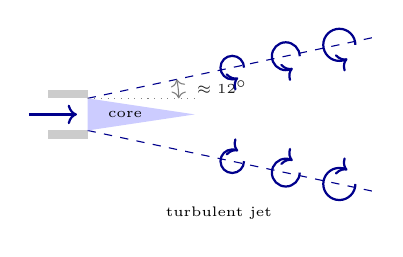
\begin{tikzpicture}[x=0.68cm,y=0.68cm]
  % nozzle
  \fill[gray!40] (0,0.30) rectangle (0.75,0.46);
  \fill[gray!40] (0,-0.30) rectangle (0.75,-0.46);
  \draw[->,thick,blue!55!black] (-0.35,0) -- (0.55,0);
  % spreading shear layers, half-angle ~12 degrees
  \draw[blue!55!black,dashed] (0.75,0.30) -- (6.1,1.44);
  \draw[blue!55!black,dashed] (0.75,-0.30) -- (6.1,-1.44);
  % potential core wedge
  \fill[blue!20] (0.75,0.30) -- (0.75,-0.30) -- (2.75,0) -- cycle;
  \node[font=\tiny,anchor=west] at (0.95,0) {core};
  % spreading angle, measured from the nozzle lip
  \draw[gray,dotted] (0.75,0.30) -- (2.75,0.30);
  \draw[<->,gray] (2.45,0.30) arc (0:12:1.70);
  \node[font=\tiny,anchor=west,gray!25!black] at (2.60,0.50) {$\approx12^\circ$};
  % roll-up vortices in the shear layers
  \foreach \xc/\rr in {3.45/0.22, 4.45/0.26, 5.45/0.30}{%
    \pgfmathsetmacro{\yc}{0.30+(\xc-0.75)*0.2126}
    \draw[->,blue!55!black,thick] ({\xc+\rr},{\yc}) arc (0:300:\rr);
    \draw[->,blue!55!black,thick] ({\xc+\rr},{-\yc}) arc (0:-300:\rr);
  }
  \node[font=\tiny,anchor=north] at (3.2,-1.55) {turbulent jet};
\end{tikzpicture}

{\scriptsize Schematic (instructor's course notes).}

\end{columns}


\end{frame}

% ---------------- Big-picture: model/optimize/control ----------------
\begin{frame}{End goal: predict, optimize, and control}
\begin{itemize}
  \item Engineering and scientific aim: develop models that predict how outcomes change with design knobs.
  \item Examples: increase lift, decrease drag, enhance mixing, reduce noise.
  \item Control: actively manipulate flow for better performance.
\end{itemize}

\vspace{0.5em}
\centering
    \includegraphics[width=0.65\linewidth]{pictures/5-1/wing-fin.jpg}

    \vfill
    {\footnotesize Source: Ball, P. Wing and fin motions share universal principles. Nature (2014).}
    
\end{frame}

% =====================================================================
% OPTIONAL / IF TIME (adds ~2--4 minutes)
% =====================================================================

\begin{frame}{Preview: Reynolds decomposition}

Recall the Navier-Stokes equations:

\begin{align*}
\frac{\partial\uu}{\partial t} + (\uu\cdot\nabla)\uu &= -\nabla \pp + \frac{1}{\Rey}\, \Delta \uu,\\
\nabla\cdot\uu &= 0.
\end{align*}

Choose an averaging operator and write the Reynolds decomposition:
\[
\uu(\bm{x},t) = \overline{\uu}(\bm{x},t) + \uu'(\bm{x},t),
\qquad \overline{\uu'}=\bm{0}.
\]
\begin{itemize}
  \item The mean may be an ensemble, spatial, phase, or time average.
  \item For statistically stationary, ergodic flow, a sufficiently long time average can represent the ensemble mean.
  \item Fluctuations $\uu'$: turbulent deviations around the mean.
\end{itemize}

\end{frame}

\begin{frame}{Why averaging became natural historically}
\begin{itemize}
  \item Before modern field measurements (e.g., PIV/laser sheets), data were often pointwise.
  \item Hot-wire anemometry: long time series at one point $\rightarrow$ build statistics.
  \item Averaging is both practical (data) and useful (reduced modeling complexity).

  \vspace{0.5em}
\centering
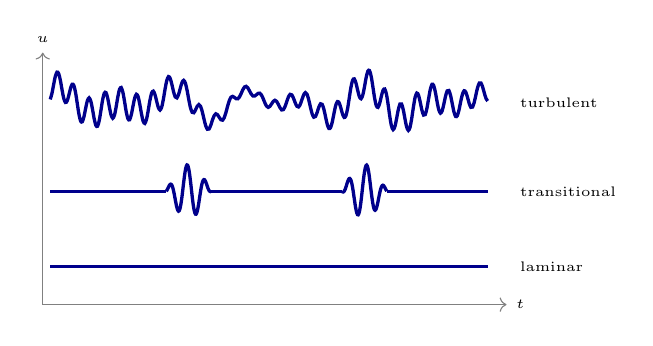
\begin{tikzpicture}[x=0.95cm,y=0.80cm]
  \draw[->,gray] (0.05,0.05) -- (6.25,0.05) node[right,font=\tiny,black] {$t$};
  \draw[->,gray] (0.05,0.05) -- (0.05,4.05) node[above,font=\tiny,black] {$u$};
  % laminar: flat
  \draw[very thick,blue!55!black] (0.15,0.65) -- (6.0,0.65);
  \node[font=\tiny,anchor=west] at (6.3,0.65) {laminar};
  % transitional: flat with two bursts
  \draw[very thick,blue!55!black] (0.15,1.85) -- (1.70,1.85);
  \draw[very thick,blue!55!black,smooth,samples=70,domain=1.70:2.30]
    plot ({\x},{1.85+0.42*sin(1500*\x)*sin(180*(\x-1.70)/0.60)});
  \draw[very thick,blue!55!black] (2.30,1.85) -- (4.05,1.85);
  \draw[very thick,blue!55!black,smooth,samples=70,domain=4.05:4.65]
    plot ({\x},{1.85+0.42*sin(1500*\x)*sin(180*(\x-4.05)/0.60)});
  \draw[very thick,blue!55!black] (4.65,1.85) -- (6.0,1.85);
  \node[font=\tiny,anchor=west] at (6.3,1.85) {transitional};
  % turbulent: broadband
  \draw[very thick,blue!55!black,smooth,samples=260,domain=0.15:6.0]
    plot ({\x},{3.25+0.30*sin(1000*\x)*cos(731*\x)+0.16*sin(433*\x)+0.09*cos(1637*\x)});
  \node[font=\tiny,anchor=west] at (6.3,3.25) {turbulent};
\end{tikzpicture}

{\scriptsize Sketch of laminar, transitional, and turbulent velocity signals recorded at a point (e.g.\ by a hot-wire anemometer). Schematic (instructor's course notes).}

\end{itemize}

\end{frame}

\begin{frame}{Takeaways}
\begin{itemize}
  \item Turbulence is hard to define, but easy to recognize by its \textbf{fingerprint}:
  \[
  \text{3D} \;+\; \text{multi-scale} \;+\; \text{unsteady} \;+\; \text{mixing}.
  \]
  \item The Navier--Stokes equations remain the anchor; $\Rey$ is an important control parameter, not a complete state label.
  \item Coherent structures and intermittency mean turbulence is \textbf{not} pure randomness.
  \item Canonical flows are how we build understanding and models.
\item What's next: Reynolds averaging/closure.
\end{itemize}
\end{frame}

\begin{frame}{Selected references}
\footnotesize
\begin{itemize}
  \item O. Reynolds, ``An experimental investigation of the circumstances which determine whether the motion of water shall be direct or sinuous,'' \emph{Phil. Trans. R. Soc. Lond.} \textbf{174} (1883), 935--982. \href{https://doi.org/10.1098/rstl.1883.0029}{doi:10.1098/rstl.1883.0029}.
  \item A. N. Kolmogorov, ``The local structure of turbulence in incompressible viscous fluid for very large Reynolds numbers,'' \emph{Proc. R. Soc. A} \textbf{434} (1991 translation), 9--13. \href{https://doi.org/10.1098/rspa.1991.0075}{doi:10.1098/rspa.1991.0075}.
  \item R. H. Kraichnan, ``Inertial ranges in two-dimensional turbulence,'' \emph{Phys. Fluids} \textbf{10} (1967), 1417--1423. \href{https://doi.org/10.1063/1.1762301}{doi:10.1063/1.1762301}.
  \item K. Avila, D. Moxey, A. de Lozar, M. Avila, D. Barkley, and B. Hof, ``The onset of turbulence in pipe flow,'' \emph{Science} \textbf{333} (2011), 192--196. \href{https://doi.org/10.1126/science.1203223}{doi:10.1126/science.1203223}.
  \item S. B. Pope, \emph{Turbulent Flows}, Cambridge University Press (2000).
\end{itemize}
\end{frame}

\end{document}
